\documentclass{article}

\usepackage{ragged2e}
\usepackage{graphicx}
\usepackage{amsmath}
\usepackage{siunitx}
\usepackage{hyperref}

% This stuff is for figures, don't copy-paste
\usepackage{float}
\DeclareGraphicsExtensions{.png, .pdf}
%\DeclareGraphicsExtensions{.pdf, .png}

\renewcommand{\c}[1]{\texttt{#1}}

\begin{document}

%\begin{flushright}
    \noindent
    Rodrigo Becerril Ferreyra\\
    CECS 346 Section 03\\
    Lab 3\\
    30 September 2020
%\end{flushright}

%\addcontentsline{toc}{section}{Introduction}
\section{Introduction} The purpose of this lab is to extend
the previous lab (Lab 2) in preparation for Project 1, where
we will be tasked to create a fully-functional traffic light
controller. Specifically, we were tasked with the following:
add a second set of lights (for a total of six LEDs) to
simulate north/south and east/west traffic lights,
add a reliable delay using
the SysTick timer functionality, and
implement a finite state machine (FSM) controller to
handle switching the lights. The timer will be responsible
for controlling how long a given light is held for. The
FSM will handle the current state, next state, and outputs
based on the current state (a Moore FSM). The functionality
of Lab 3 is as follows:

\begin{itemize}
    \item If no switches are pressed, stay on the current state.
    \item If the NS (north/south) switch is pressed, make the NS light green and the EW (east/west) light red.
    \item If the EW switch is pressed, make EW green and NS red.
    \item If both switches are pressed, rotate between green on EW and NS.
    \item The default state on reset is NS = red, EW = green.
\end{itemize}

The delay for holding a green light is \SI{2}{s}, and the
delay for holding a yellow light is \SI{1}{s}. Lights switch as
usual (green, yellow, red, green, etc.).

\section{Hardware} The hardware in this Lab is simply an
extension of the last lab. We are again using pins \c{B[1:0]}
as switch inputs (with \SI{10}{\kilo\ohm} pull-down resistors),
and pins \c{E[2:0]} as outputs for the NS set of lights.
We are adding pins \c{E[5:3]} as outputs for the EW set of
lights as an extension for this Lab. All LEDs source less
than \SI{2}{\milli\ampere} of current from the board and
are hooked up to \SI{690}{\ohm} (\(\SI{470}{\ohm}
+ \SI{220}{\ohm}\)) current-limiting resistors.

\section{Software} The software was easy to extend from Lab 2.

The SysTick timer is a hardware timer separate from the
General-Purpose timers found on the board's microcontroller.
It only has three registers to its name, and is simple to
initialize.
It is a 24-bit count-down timer intended for light-use
applications such as delay. Before SysTick, we had to use
an empty \c{for} loop in order to achieve an approximate
delay time. The number of iterations had to be experimentally
found, and that was only to a certain degree of accuracy. With
the SysTick timer, we know by the datasheet exactly how fast
the timer counts down: at \SI{16}{\mega\hertz}, which is
equivalent to one count every \SI{62.5}{\nano\second}.
From this, one can calculate the amount of counts needed to
achieve a \SI{1}{\micro\second} delay (which is \(16-1\) since
zero is also counted), and from there one can create a loop
which runs this delay \num{1000000} times creating a precisely
\SI{1}{\second} delay.

The finite state machine was implemented using a \c{struct}.
A \c{struct} is similar to a class in object-oriented
programming languages, as it includes variables inside of it
(but cannot contain function definitions). Together with the
\c{typedef} keyword, it can be used similarly to a class.
The FSM ``skeleton'' has output, delay, and next state variables;
we only initialized one FSM, but we could have initialized more
to provide alternate decision-making functionalities if we wished.
The FSM was created to the specifications above (See Section 1).

\pagebreak

\section{Media}
\begin{itemize}
    \item Link to video demonstration:
    \begin{itemize}
        \item \url{https://youtu.be/fB_rXp9ZSGE}
    \end{itemize}
    \item Picture of embedded system:
    \begin{figure}[H]
        \centering
        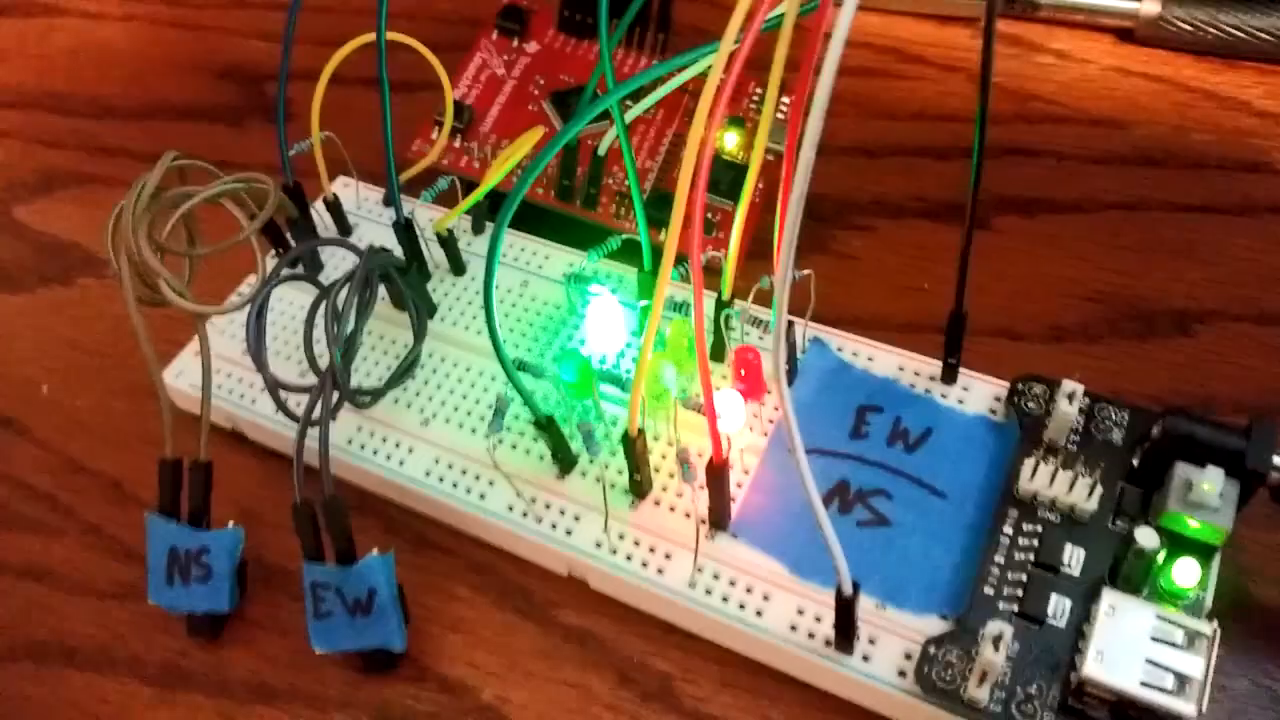
\includegraphics[height=162pt]{Images/embeddedsystem}
    \end{figure}
    \item Hardware schematic:
    \begin{figure}[H]
        \centering
        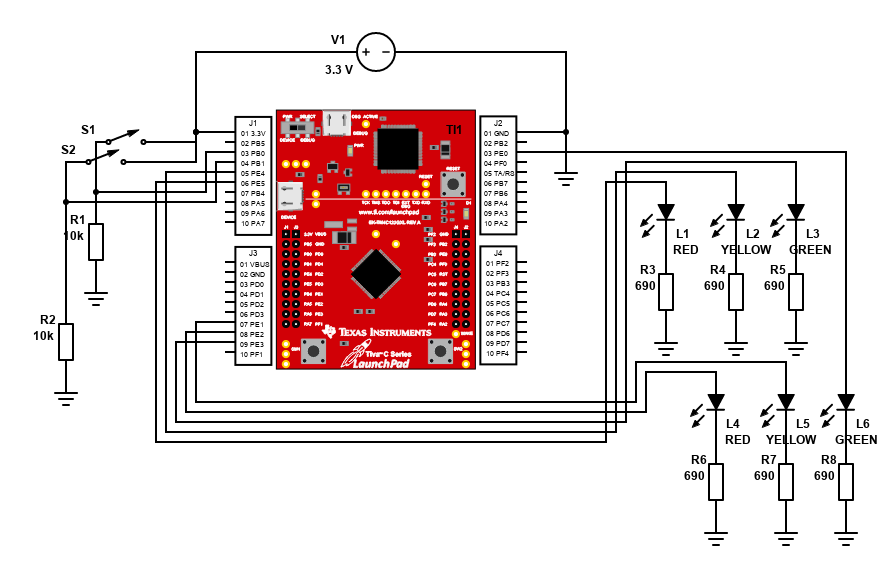
\includegraphics[height=162pt]{Images/schemeit-project}
    \end{figure}
\end{itemize}

\end{document}
